%*****************************************
\chapter{Grundlagen}\label{ch:preliminaries}
%*****************************************
% \section*{Inhalte des Kapitels}
% - Taxonomie von Ammus (\citet{ammus}) % DONE
% - Transformer Architektur (\citet{attention}) % DONE

% - Neuronales Netz (https://katalog.ub.uni-leipzig.de/Record/0-1066754535) % DONE
% - Activation Functions (https://katalog.ub.uni-leipzig.de/Record/0-1066754535) % DONE
% - Backpropagation (https://katalog.ub.uni-leipzig.de/Record/0-1066754535)% DONE
% - Training eines Modells % DONE
%     - Batching % DONE
%     - Optimizer % DONE
%     - Learning Rate % DONE

% - Feed-Forward Netze
% - Multi-Head Attention
% - Encoder und Decoder

% - Input embeddings = Embeddings
% - Positional Embeddings
% - Tokenization % DONE
%     - Byte Pair Encoding % DONE


% Sprachmodell Definition (Was ist das)

% - Autoregressive Modelle % DONE
%     - Self-supervised Learning % DONE
%     - Pretraining
%     - continual Pretraining
%     - Decoder-Based % DONE
%     - ZeroShot / FewShot

% - Weiterentwicklungen
%     - Deep Residual Connections % DONE
%     - DropOut   % DONE

% Wissen, Information, Daten (Winter)
% FScore, Precision, Recall, Micro und MacroF1 (QUALD9)
% Question Answering (Aggregation, erst FScore für Frage, dann Durchschnitt, oder andersrum)
% API, Overfitting
%************ Sprachmodelle
Zum Verständnis der in \cref{sec:zielsetzung} genannten Ziele und Ausführungen dieser Arbeit werden in diesem Kapitel Grundlagen zu den verwendeten Begriffen und Konzepten geschaffen.
Das Kapitel gliedert sich in eine allgemeine Definition von Sprachmodellen in \cref{sec:sprachmodelle} mit einer genaueren Erläuterung der Transformer-spezifischen Architektur.
Danach folgt eine kurze Einführung in das Thema Neuronale Netze, in der die Funktionsweise von Neuronalen Netzen näher erläutert wird.
Abschließend werden einige Begriffe aus der Medizinischen Informatik und der Datenverarbeitung in \cref{sec:Datenverarbeitung} erläutert.

\section{Sprachmodelle}\label{sec:sprachmodelle}

\begin{definition}\label{def:sprachmodell}
   \textbf{Sprachmodelle} sind neuronale Netze, welche menschliche Sprache verstehen und darauf reagieren.
\end{definition}
Sprachmodelle basieren auf künstlicher Intelligenz und werden in der Regel durch maschinelles Lernen trainiert.
Sie werden in einer Vielzahl von Anwendungen eingesetzt, wie z.B. in der Übersetzung,
Textgenerierung, Spracherkennung und Textklassifikation.

\begin{definition}\label{def:autoregressive-sprachmodelle}
    \textbf{Autoregressive Sprachmodelle} sind Sprachmodelle, die Texte generieren,
    indem sie die Wahrscheinlichkeit von Wörtern oder Zeichen in einer Sequenz vorhersagen.
\end{definition}

Autoregressive Modelle basieren auf der Annahme, dass jedes Element in der Sequenz von den vorhergehenden Elementen abhängt.
In einem autoregressiven Sprachmodell wird die generative Wahrscheinlichkeit des nächsten Elements in der Sequenz geschätzt.
Die Ausgabe im Kontext von Decoder-basierten Modellen ist daher eine Wahrscheinlichkeitsverteilung über das mögliche nächste Element.
Das wahrscheinlichste Element wird dann der Sequenz hinzugefügt, und der Prozess wird wiederholt, bis die Sequenz vollständig ist.
Üblicherweise werden autoregressive Sprachmodelle auf großen Textdatenmengen trainiert, um die statistischen Zusammenhänge in den Trainingsdaten zu erfassen.

\subsection{Transformer-Modelle}\label{sec:grundlagen:transformer}

\begin{definition}\label{def:transformer-modell}
    Ein \textbf{Transformer-Modell} ist ein Sprachmodell, das auf der Transformer-Architektur von \citet{attention} basiert.
\end{definition}
Im Gegensatz zu früheren Sprachmodellen, die auf rekurrenten oder faltenden neuronalen Netzen basieren, verwendet der Transformer einen Aufmerksamkeitsmechanismus, um die Beziehungen zwischen Wörtern in einem Satz zu modellieren.
Transformer-Modelle bestehen aus einer Stapelung von Encoder- und Decoder-Schichten, wobei der Encoder dazu dient, Kontextinformationen aus der Eingabe zu extrahieren,
während der Decoder die Ausgabe des Encoders verwendet, um die gewünschte Aufgabe zu lösen.
Die Architektur eines Transformators ist in \cref{bild:transformer} dargestellt.\\

\begin{figure}[ht]
    \centering
    \includegraphics[width=0.8\textwidth]{zeichnungen/transformer.png}
    \caption{Die Transformer-Modell Architektur \citep{attention}}
    \label{bild:transformer}
\end{figure}

Die erste schriftliche Erwähnung des Transformer-Modells sowie die Einführung der beiden Teilmodelle Encoder und Decoder findet sich in \citet{attention}.
Die hier beschriebene bidirektionale Architektur bildet die Grundlage für alle darauf aufbauenden Modelle und Weiterentwicklungen.
Die Basisarchitektur wurde für verschiedene Anwendungen stark modifiziert.
Seit 2017 gibt es grundlegende Unterschiede in den Modellen und deren Möglichkeiten.
Aus diesem Grund haben \citet{ammus} eine Taxonomie der Transformer-basierten vortrainierten Sprachmodelle eingeführt.
Diese Taxonomie wird hier zur Beschreibung weiterer Architekturen und Methodiken verwendet.\\

Neben dem Grundbaustein eines Transformers --- dem Aufmerksamkeitsmechanismus --- sind zwei wichtige Modifikationen gegenüber normalen neuronalen Netzen in Transformer eingeflossen: Residuale Verbindungen und Dropout.\\

\subsubsection{Residuale Verbindungen}

\begin{definition}\label{def:residuale-verbindungen}
    \textbf{Residuale Verbindungen} oder auch Deep Residual Connections, sind direkte Verbindungen zwischen Eingabe und Ausgabe und überspringen somit eine oder mehrere Schichten eines \ac{nn}.
\end{definition}
Residuale Verbindungen als Level-Normalisierung ändern das Ziel eines \ac{nn}s, behalten aber die gleichen Ausgaben durch ihre Level-Normalisierung bei.
Dieses Konzept wurde erstmals in \citet{deep_residual} eingeführt und bietet eine Lösung für ein grundlegendes Problem von großen, mehrschichtigen Transformer-Modellen.
Bereits 2016 wurde im Bereich der Bilderkennung festgestellt, dass sich die Korrektheit von Modellen mit zunehmender Tiefe sättigt und sich dann rapide verschlechtert, wenn dieses Modell weiter trainiert wird.
Dies setzte eine praktische Grenze für die Tiefe von \ac{nn}s und verhinderte somit die Lösung komplexerer Probleme mit größeren Modellen.
\citet{deep_residual} beschreiben eine Lösung durch die genannten Residuen, die normale \ac{nn} einfach ersetzen können, und zeigen auch die Effizienz dieser Methode.\\

\subsubsection{Dropout}

Die Einführung von Dropouts ist die zweite wichtige Änderung zur Weiterentwicklung der Transformer-Architektur.
\begin{definition}\label{def:dropout}
    \textbf{Dropout} ist eine Methode, die die Trainingszeit von \ac{nn}s verkürzt und die Generalisierung verbessert.
    \citet{dropout} beschreiben die Methode als das zufällige Aussetzen von Neuronen unabhängig von der Eingabe in einem \ac{nn} während des Trainings. 
\end{definition}
Durch das Aussetzen von Neuronen wird das \ac{nn} gezwungen, sich nicht auf andere Neuronen zu verlassen und somit eine bessere Generalisierung zu erreichen.
Das Aussetzen erfolgt nur während des Trainings und nicht während der Inferenz.
Die Methode wurde 2014 eingeführt und ist seitdem ein fester Bestandteil von \ac{nn}s.\\

\subsubsection{Modellarten von Transformer-Modellen}

Basierend auf der eingeführten Transformer-Architektur wurden verschiedene Modelltypen entwickelt, die nur Teile der Architektur nutzen und sich in ihrer Funktionsweise unterscheiden.

\begin{definition}\label{def:encoder-basierte-modelle}
    \textbf{Encoder-basierte Modelle} sind Sprachmodelle, die hauptsächlich auf der Encoder-Architektur basieren.
    Sie wurden entwickelt, um Eingabesequenzen zu verarbeiten und eine kompakte Repräsentation (auch Kontextvektor genannt) zu erzeugen.
\end{definition}
Die zentrale Komponente eines Encoder-basierten Modells ist der Encoder.
Er empfängt die Eingabesequenz und lernt schrittweise, die strukturellen und semantischen Informationen zu erfassen.
Die so erzeugte Repräsentation des Encoders kann von anderen Modulen oder Schichten des Modells verwendet werden, um verschiedene Aufgaben 
wie z.B. die Klassifikation zu lösen.
Encoder-basierte Modelle haben in der Regel keine Decoder-Schicht.\\

\begin{definition}\label{def:decoder-basierte-modelle}
    \textbf{Decoder-basierte Modelle} sind Sprachmodelle, die auf einer speziellen Architektur basieren, bei der der Decoder eine zentrale Rolle spielt.
    Der Decoder ist eine Komponente, die darauf spezialisiert ist, aus einer gegebenen Eingabe eine sinnvolle und kohärente Ausgabe zu erzeugen.
\end{definition}
Im Zusammenhang mit der Textgenerierung erhält der Decoder normalerweise eine Sequenz von Vektoren als Eingabe, die von einem Encoder-Modul erzeugt wurde.
Bei der Textgenerierung kann der Decoder aus einer gegebenen Ausgangssequenz fortlaufend neue Wörter oder Sätze generieren, um einen zusammenhängenden Text zu erzeugen.

\subsection{Transformer-spezifische Architekturen}

\begin{definition}\label{def:self-attention-mechanismus}
    Der \textbf{Self-Attention-Mechanismus} ist ein zentrales Konzept in der Transformer-Architektur und beschreibt die Gewichtung der Eingabesequenz auf Basis eines aktuellen Tokens.
\end{definition}
Hier wird ein Eingabevektor in drei separate Vektoren transformiert:
Den Abfragevektor (engl. Query), den Schlüsselvektor (engl. Key) und den Wertvektor (engl. Value).
Anschließend wird die Ähnlichkeit zwischen dem Abfragevektor und dem Schlüsselvektor berechnet,
um die Aufmerksamkeitsgewichte zu erhalten.
Die Aufmerksamkeitsgewichte geben an, wie wichtig jeder Wertvektor für die Berechnung eines gewichteten
Durchschnitts ist. Die gewichteten Wertvektoren werden schließlich summiert, um den Ausgabevektor zu erhalten.
Die Self-Attention Mechanismen ermöglichen es den Modellen, komplexe Abhängigkeiten zwischen den Elementen einer Eingabesequenz zu erfassen.\\

\begin{definition}\label{def:multi-head-attention}
    \textbf{Multi-Head Attention} beschreibt den Ersatz eines einzelnen Self-Attention-Mechanismus in der Transformer-Architektur durch mehrere parallel arbeitende Self-Attention-Mechanismen.
\end{definition}
Beim Multi-Head Attention-Verfahren werden die Anfrage, der Schlüssel und der Wert $h$-mal linear auf mehrere Versionen projiziert und parallel berechnet. Die Ausgabe wird dann verkettet und erneut linear projiziert, um den Ausgabevektor zu erhalten. Multi-Head Attention ermöglicht es dem Modell, verschiedene Repräsentationsteilräume der Eingabe an verschiedenen Positionen zu erfassen.

\begin{definition}\label{def:feed-forward-netz}
    Ein \textbf{Feed-Foward-Netz} ist eine Art künstliches neuronales Netz, das aus mehreren Schichten besteht und Informationen nur vorwärts von der Eingabe zur Ausgabe fließen lässt.
\end{definition}
Feed-Foward-Netze haben keine zyklischen Verbindungen oder Rückkopplungsschleifen.
Sie dienen in Transformern neben den Aufmerksamkeitsnetzen als einzige zweite Komponente der Architektur.
Sie enthalten das erlernte Faktenwissen des Modells durch sogenannte Wissensneuronen \citep{knowledge_neurons}.\\

\subsection{Eigenheiten von Transformer-Modellen}
\begin{definition}\label{def:zeroshot-oneshot-multishot}
    Die Bezeichnungen \textbf{ZeroShot, OneShot} und \textbf{MultiShot} beziehen sich auf die Inferenz von Modellen.
    Die Eingabe enthält hier Beispielaufgaben, bevor die eigentliche Aufgabe gestellt wird.
\end{definition}
Insbesondere bei \ac{qa}-Aufgaben und Textgenerierungen werden diese Methoden häufig verwendet.
Bei der Beantwortung von Fragen können die Eingaben mehrere Beispielfragen und deren Antworten enthalten, bevor die eigentliche Frage gestellt wird.
Dadurch kann das Modell die Formatierung und Art der Aufgabe aus dem Kontext erkennen und bessere Antworten liefern.
\mbox{ZeroShot} bedeutet, dass das Modell keine Trainingsbeispiele erhält, um eine bestimmte Aufgabe zu lösen.
OneShot bedeutet, dass das Modell nur ein Trainingsbeispiel erhält, um eine bestimmte Aufgabe zu lösen.
MultiShot bedeutet, dass das Modell mehrere Trainingsbeispiele erhält.


\begin{definition}\label{def:parameterformate}
    \textbf{Parameterformate} sind Variableneinheiten von lernbaren Parametern.
    Häufig verwendet werden \enquote{Float16} und \enquote{Float32}.
\end{definition}
Sprachmodelle enthalten eine große Anzahl lernbarer Parameter (wie z.B. Gewichte und Bias),
sowie Zwischenwerte, die während der Inferenz berechnet werden.
Diese Werte können in unterschiedlichen Formaten gespeichert werden.
Gängige Formate sind hier \enquote{Float16} und \enquote{Float32}.
Float steht hier für Floating Value und stellt eine Fließkommazahl dar.
Die Zahl hinter Float gibt die Anzahl der Bits an, die zur Darstellung der Zahl verwendet werden.
Eine höhere Anzahl von Bits bedeutet eine höhere Genauigkeit, aber auch einen höheren Speicherbedarf.

\begin{definition}\label{def:continual-pretraining}
    \textbf{Continual Pretraining} beschreibt den Prozess des kontinuierlichen, selbstüberwachten Trainings eines vortrainierten Modells.
\end{definition}
Beim Continual Pretraining werden nur die Hyperparameter des Modells angepasst und neue Datensätze verwendet, während auf die bereits erlernten Parameter des Modells aufbauend weitertrainiert wird.

%************ Transformer-Spezifische Eingaben

\subsection{Eingaben von Transformer-Modellen}
\begin{definition}\label{def:token}
    Ein \textbf{Token} repräsentiert eine Teilmenge eines Wortes und wird in Transformer-Modellen verwendet, um die Eingabe in logische Einheiten zu unterteilen.
\end{definition}
Transformer-Modelle können Eingaben nicht ohne zusätzliche Umwandlung verarbeiten.
Neben der Erzeugung von Eingabevektoren muss die Eingabe zunächst in kleinere Einheiten, so genannte Tokens, zerlegt werden.
Verschiedene ältere Modelle verwenden dazu Wörter oder Symbolunterteilungen.
Dies ist jedoch problematisch.\\

Durch die Zerlegung der Eingaben in Symbole ist zwar das Vokabular kleiner, welches zu schnelleren Trainingsdurchläufen führt, jedoch muss das Modell vor dem Erlernen von Wortzusammenhängen, Satzstrukturen und Sachverhalten zunächst die Bedeutung der Wörter und deren Zusammensetzung aus Symbolen erlernen.
Dadurch geht ein großer Teil der Trainingszeit für das Erlernen der Sprache verloren, was die endgültige Leistungsfähigkeit der Modelle stark einschränkt \citep{bpe}.\\

\begin{definition}\label{def:vokabular}
    Das \textbf{Vokabular} eines Modells ist die Menge aller Token, die das Modell als individuelle Einheiten erkennt. Die Größe des Vokabulars bestimmt die Größe der Input-Embeddings und begrenzt somit die Größe der Eingaben.
\end{definition}

Eine logische Schlussfolgerung wäre hier die Verwendung von Wörtern oder sogar Phrasen als Tokens.
Mit zunehmender Größe der Datensätze, die zum Training der Modelle verwendet werden, wächst das Vokabular enorm an.
Dies führt zu einer starken Verlangsamung der Trainingsläufe und zu sehr großen Modellen ohne Leistungsvorteil.
Wörter mit gleichem Wortstamm oder ähnlicher Bedeutung aufgrund grammatikalischer Regeln (Plural, Genus, Tempus) müssen vom Modell zunächst als \enquote{gleiches Wort} gelernt werden.
Daher hat sich die Unterteilung von Wörtern in Teilwörter als Standard durchgesetzt.

\subsubsection{Byte Pair Encoding}
\begin{definition}\label{def:bpe}
    \textbf{Byte Pair Encoding} ist ein Algorithmus, der iterativ ein Vokabular basierend auf der Häufigkeit von Symbolkombinationen in einem Datensatz aufbaut.
    Die Vokabulargröße ist der einzige Parameter.
\end{definition}
\citet{bpe} schlugen zu diesem Zweck die Verwendung von \ac{bpe} vor.
Die Unterteilung von Wörtern in Untergruppen von Wörtern hat bereits zu erheblichen Verbesserungen bei der Übersetzung von Sätzen geführt.
Sie hat sich aber auch in anderen Bereichen und Aufgaben wie der Textgenerierung, der Textklassifikation und der Analyse von Emotionen durchgesetzt.
Die Unterteilung von Wörtern ist hier eher als das Zusammensetzen von kleinen Teilwörtern zu verstehen.
Ausgehend von einem Vokabular, das aus allen Symbolen eines Alphabets besteht, wird dieses durch Zusammenfügen (engl. \enquote{Merge}) der Symbole erweitert, deren Kombination im Datensatz am häufigsten vorkommt.
Dieser Vorgang wird so lange wiederholt, bis die gewünschte Anzahl von Teilwörtern erreicht ist.
Die Anzahl der Teilwörter ist ein Hyperparameter, der je nach Modell und Datensatz variiert.\\

Die Unterteilung von Wörtern in Teilwörter hat den Vorteil, dass die Größe des Vokabulars nicht mit der Größe des Datensatzes wächst.
Dies führt zu einer schnelleren Eingabeverarbeitung und einer besseren Generalisierung der Modelle.
Die Unterteilung von Wörtern in Teilwörter hat jedoch auch Nachteile.
Sie ist nicht eindeutig, d.h. ein Wort kann in verschiedene Mengen von Teilwörtern zerlegt werden.
Dies führt zu einer größeren Anzahl möglicher Eingaben, die das Modell lernen muss.\\

Ein weiterer Nachteil ist, dass die Zerlegung von Wörtern in Teilwörter nicht immer sinnvoll ist.
So kann es vorkommen, dass ein Wort in Teilwörter zerlegt wird, die in der Sprache nicht existieren.
Dies wiederum minimiert die Verallgemeinerbarkeit der Modelle.
Ein Beispiel hierfür ist das Wort \enquote{Datensatz}.
Eine sinnvolle Unterteilung wäre hier \enquote{Daten} und \enquote{satz}, aber durch den Aufbau des Vokabulars aus den Symbolen des Datensatzes kann es vorkommen, dass das Teilwort \enquote{Daten} nicht die notwendige Häufigkeit besitzt und somit nicht im Vokabular vorhanden ist.
Daher muss auch dieses Wort zerlegt werden, z.B. in \enquote{Dat} und \enquote{en}.
Beide Teilwörter haben in der deutschen Sprache keine Bedeutung, werden aber durch das Modell mit Bedeutung versehen und in Beziehung zu anderen Wörtern gesetzt.
Dies führt zu einer unverständlichen Bedeutungsannotation von Teilwörtern und verschlechtert sowohl die Leistung als auch die Nachvollziehbarkeit des Modells und erschwert die Forschung an den Modellen.

\subsubsection{Eingabevektoren}

\begin{definition}\label{def:input-embeddings}
    \textbf{Input Embeddings} sind eine Darstellung der Eingabedaten in Form von Token in einem dichten Vektorraum.
\end{definition}
Die Repräsentation von Token in einem Vektorraum muss erlernt werden und ermöglicht es,
Token, die semantische Ähnlichkeiten oder Beziehungen zueinander aufweisen, geometrisch nahe beieinander zu platzieren.
Dadurch ist nicht nur das Token selbst, sondern auch die Beziehung zu anderen Tokens bekannt. Mit zunehmender Größe des Vokabulars müssen auch die Dimensionen der Input Embeddings vergrößert werden, da es sonst zu ungewollten Kollisionen zwischen Tokens kommen kann.

\begin{definition}[Positional Encodings]\label{def:positional-encodings}
    \textbf{Positional Encodings} stellen sogenannte relative und absolute Positionen der Token in der Eingabe dar.
\end{definition}
Relative und absolute Positionen von Token innerhalb einer Eingabe werden in einem Vektorraum dargestellt und ermöglichen es dem Modell, die Positionen der Token zu berücksichtigen.
Positional Encodings können gelernt oder berechnet werden und werden nur in Kombination mit Input Embeddings verwendet.

\section{Neuronale Netze}\label{sec:neuronale-netze}
Um die Architektur des Transformers zu verstehen, ist es notwendig, die Grundlagen neuronaler Netze zu kennen.
Neuronale Netze wurden erstmals 1943 von \citet{neuronal_networks_first} beschrieben und haben seitdem viele Veränderungen und Verbesserungen erfahren.
Eine Beschreibung der grundlegenden Techniken findet sich in \citet{neuronale-netze}.
Aufbauend auf diesem Buch wird im Folgenden ein Überblick über die Funktionsweise von Neuronalen Netzen gegeben.\\

\subsection{Architektur}
Neuronale Netze ahmen die Funktionsweise des menschlichen Gehirns mit Hilfe mathematischer Gleichungen nach.
Ein Netz besteht aus einer Anzahl von Neuronen, die sowohl Eingangs- als auch Ausgangsverbindungen zu anderen Neuronen haben.
Neuronen haben die Eigenschaft, von bestimmten Eingängen einen Impuls an die Ausgänge zu senden, wenn ein Schwellenwert überschritten wird.
Im Gegensatz zum Gehirn sind normale neuronale Netze jedoch logischer aufgebaut.
Die Neuronen sind in Schichten angeordnet, wobei die erste Schicht die Eingangsschicht mit den Eingangsneuronen $E_N$ und die letzte Schicht die Ausgangsschicht mit den Ausgangsneuronen $A_N$ ist.
Die Schichten zwischen diesen beiden Grenzen werden als versteckte Schichten (engl. Hidden Layers) mit Neuronen $H^L_N$ bezeichnet.\\

\begin{figure}
    \centering
    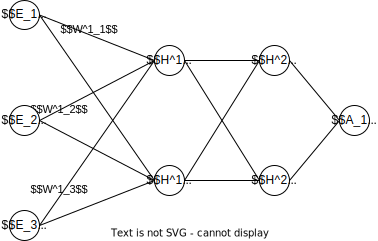
\includegraphics[width=\textwidth]{zeichnungen/nn.png}
    \caption{Beispiel-Aufbau eines Neuronalen Netzes mit 3 Eingangsneuronen, 4 versteckten Neuronen und einem Ausgangsneuronen.}\label{nn_simple}
\end{figure}

\cref{nn_simple} zeigt eine Beispielkonfiguration mit 3 $E_N$, hier bezeichnet als $E_1,E_2,E_3$, zwei versteckten Schichten mit je zwei $H^L_N$, hier bezeichnet als $H^1_1, H^1_2$ und $H^2_1, H^2_2$ und einem Ausgangsneuron $A_1$.
Die Neuronen sind mit sogenannten Gewichten $W_N$ verbunden. Man spricht hier von einer Vorwärtsverbindung.
Das bedeutet, dass die Eingaben durch die Schichten in Richtung Ausgabe weitergereicht werden, aber nicht zurück zur Eingabe fließen können.
Im Beispiel in \cref{nn_simple} sind diese Verbindungen vollständig.
Jedes Neuron einer Schicht hat eine Verbindung zu jedem Neuron der nächsten Schicht.
Hier nicht gezeigt, hat jedes Neuron auch eine Eingangsverbindung von einem Bias $B_N$.

\subsection{Funktionsweise}
Die Anwendung des Neuronalen Netzes erfolgt in zwei Schritten.
Zuerst wird eine Eingabe in die Eingangsneuronen $E_N$ eingegeben.
Diese Eingabe wird durch die Schichten weitergegeben, bis sie in der Ausgabeschicht $A_N$ ankommt.
Jetzt muss das Ergebnis interpretiert werden. Dieser Vorgang wird auch als Inferenz bezeichnet.\\\
\begin{definition}\label{def:inferenz}
    \textbf{Inferenz} beschreibt den Prozess, bei dem ein Modell aufgrund der gelernten Parameter eine Vorhersage trifft.
\end{definition}

Ein Anwendungsbeispiel wäre die Erkennung von handgeschriebenen Zahlen.
Die Eingabe wäre hier ein Bild der Ziffer, das in ein neuronales Netz eingespeist wird.
Jedes Neuron repräsentiert den Grauwert eines Pixels im Bereich $[0,1]$.
Die Ausgabe stellt die erkannte Ziffer dar.
Für jede mögliche Ziffer (0-9) gibt es ein Ausgangsneuron, das vom neuronalen Netz einen Wert zwischen 0 und 1 erhält.
Das Neuron mit dem höchsten Ausgang repräsentiert die erkannte Ziffer.\\

Ein Berechnungsbeispiel für das erste Neuron der ersten versteckten Schicht $H^1_1$ sieht wie folgt aus:
\begin{equation}
    H^1_1=ReLU(W^1_1\cdot E_1 + W^1_2\cdot E_2 + W^1_3\cdot E_3 + B^1_1)
\end{equation}
$W^1_N$ stellen hier die Gewichte der ersten Schicht dar.
Gewichte sind Parameter, die während des Trainings eines Netzes angepasst werden, um eine optimale Ausgabe von $A_N$ zu erhalten.
Diese Parameter werden auch als lernbare Parameter bezeichnet.\\

\begin{definition}\label{def:lernbare-parameter}
    Ein \textbf{Lernbarer Parameter} ist ein Parameter, der zufällig initialisiert wird und während des Trainings angepasst wird.
\end{definition}

$B^1_N$ ist der Bias und ebenfalls ein lernbarer Parameter.
Alle Eingabewerte werden gemäß der Formel aufsummiert und mit Hilfe einer Aktivierungsfunktion transformiert.
Diese Aktivierungsfunktion war in früheren Netzen die Sigmoidfunktion \pcref{img:sigmoid}.
In modernen Netzen und auch in Transformer-Modellen wird hier die ReLU-Funktion \pcref{img:relu} verwendet.

\begin{figure}
    \centering
    \includegraphics[width=\textwidth]{zeichnungen/sigmoid.png}
    \caption{Die Sigmoid-Funktion $f(x) = \frac{1}{1+e^{-x}}$}\label{img:sigmoid}
\end{figure}

\begin{figure}
    \centering
    \includegraphics[width=\textwidth]{zeichnungen/relu.png}
    \caption{Die ReLU-Funktion $f(x) = \max(0,x)$}\label{img:relu}
\end{figure}

\begin{definition}\label{def:aktivierungsfunktion}
    Die \textbf{Aktivierungsfunktion} weißt jedem potentiellen Wert eines Neurons einen Wert in einem vorgegebenem Intervall zu.
    Sie ist nicht-linear und verhindert somit die Reduzierung eines Neuronalen Netzes auf eine lineare Funktion.
\end{definition}

Üblicherweise stellt eine Aktivierungsfunktion eine Transformation der Eingabewerte in einen nichtlinearen Ausgabewert zwischen 0 und 1 dar.
Dies ist jedoch nicht zwingend, da z.B. die ReLU-Funktion Werte zwischen 0 und $\infty$ ausgibt, aber schneller berechnet werden kann als die Sigmoidfunktion.
Aktivierungsfunktionen sind notwendig, um die Komplexität eines neuronalen Netzes zu erhöhen und damit seine Fähigkeit, komplexere Probleme zu lösen, zu ermöglichen.
Ohne Aktivierungsfunktion würden $A_N$ Neuronen eine Linearkombination der Eingabewerte erzeugen, wodurch nur lineare Probleme gelöst werden könnten.
Ein einfaches Beispiel ist die Berechnung der XOR-Funktion.
Die XOR-Funktion verknüpft zwei Eingaben zu einer Ausgabe. Wenn eine der beiden Eingaben 1 ist, soll auch die Ausgabe 1 sein.
Andernfalls soll die Ausgabe 0 sein.
Diese einfache Funktion kann ohne eine Aktivierungsfunktion nicht gelöst werden.\\

Die Ausgabewerte $A_N$ sind ebenfalls Werte im Bereich der Aktivierungsfunktion und nicht immer repräsentativ für das Problem, das das neuronale Netz lösen soll.
Daher werden diese Werte interpretiert und stellen häufig einen Konfidenzwert für eine bestimmte Klasse dar.
Wenn das Neuron $A_1$ den Maximalwert 1 hat, dann ist sich das Netz zu \SI{100}{\percent} sicher, dass die Eingabe der Klasse 1 entspricht.
Bei Transformern ist die Ausgabe $A_N$ ein Vektor über das gesamte Vokabular des Transformers und gibt an, inwieweit das Modell davon ausgeht, dass das jeweilige Token dem Eingabetext folgt.\\

\subsection{Training}\label{subsec:grundlagen:training}
Bevor ein neuronales Netz korrekte Ergebnisse liefern kann, muss es trainiert werden.
Training bedeutet die iterative Anpassung der Trainingsparameter, um eine möglichst gute Ausgabe zu erhalten.
Eine gute Ausgabe wird durch eine Fehlerfunktion beschrieben.
Diese Fehlerfunktion gibt einen einzelnen Wert zurück, der den Eingaben in das neuronale Netz entspricht und umgekehrt proportional zur guten Ausgabe ist.
Geometrisch stellt eine Fehlerfunktion eine mehrdimensionale Fläche dar, wobei jeder lernfähige Parameter auf einer Achse liegt und das Minimum dieser Fläche ein Optimum darstellt.
Dieses Optimum ist das Trainingsziel.
Kleine Änderungen einzelner Parameter verändern die Ausgabe der Fehlerfunktion und können somit zeigen, ob diese Änderung zu einer Verbesserung oder Verschlechterung des neuronalen Netzes geführt hat.
Hier besteht bereits die Unterscheidung zwischen einem überwachten, selbstüberwachten und unüberwachten Lernverfahren.\\

\begin{definition}\label{def:ueberwachtes-lernen}
    Bei dem \textbf{Überwachten Lernen} sind sowohl die Eingabe als auch die erwartete Ausgabe während des Trainings bekannt.
    Die verwendete Fehlerfunktion ergibt sich aus der Differenz zwischen erwarteter und tatsächlicher Ausgabe.
\end{definition}

\begin{definition}\label{def:unueberwachtes-lernen}
    Bei dem \textbf{Unüberwachten Lernen} ist während des Trainings nur die Eingabe bekannt.
    Die Fehlerfunktion muss aus dem Kontext berechnet oder abgeleitet werden.
\end{definition}

\begin{definition}\label{def:selbstueberwachtes-lernen}
    Bei dem \textbf{selbstüberwachten Lernen} ist während des Trainings nur die Eingabe bekannt.
    Die Ausgabe entspricht jedoch einem Teil der Eingabe, so dass die Fehlerfunktion berechnet werden kann.
\end{definition}

Ein Beispiel für überwachtes Lernen ist die Klassifizierung von Bildern.
Der Datensatz enthält sowohl die Bilder als auch die zugehörigen Klassen.
Daher ist die erwartete Ausgabe des Modells für ein Bild genau die Klasse.
Transformer-Modelle sind selbstüberwachende Systeme.
Hier ergibt die Eingabe die erwartete Ausgabe, da das folgende Token der Eingabe als korrekt angesehen wird.
Unüberwachte Systeme sind z.B. Agenten, die Spiele lernen.
Hier gibt es in den meisten Fällen eine Belohnungsfunktion, die angibt, wie gut das Modell gespielt hat.
Belohnungsfunktionen können beschreiben, wie weit das Auto im Spiel gefahren ist oder wie viele Punkte gesammelt wurden.\\
\subsubsection{Backpropagation}
\begin{definition}\label{def:backpropagation}
    \textbf{Backpropagation} beschreibt den Prozess der iterativen Anpassung von Gewichten und Bias auf Basis des Gradienten einer Fehlerfunktion.
\end{definition}

Eine der wichtigsten Methoden zur iterativen Anpassung von Gewichten und Bias und damit zum Training neuronaler Netze ist die Methode der Fehlerrückführung (engl. Backpropagation).
Diese Gradientenabstiegsmethode wurde erstmals 1986 von \citet{backpropagation} beschrieben und ist ausführlich in \citet{neuronale-netze} beschrieben.
Um den Rahmen dieser Arbeit nicht zu sprengen, wird hier auf eine mathematische Beschreibung verzichtet und nur die Grundidee beschrieben.\\

Die Fehlerfunktion $C$ ist eine Funktion aller Gewichte und Bias des neuronalen Netzes und seiner Ausgabe.
Ihr Minimum zu finden bedeutet, ein Optimum für das Modell zu finden.
Zu Beginn des Trainings werden alle Gewichte mit Zufallszahlen initialisiert.
Nun wird die Ausgabe des Modells berechnet und mit der erwarteten Ausgabe verglichen.
Die Funktion $C$ hat einen Gradienten $\Delta C$, der die Richtung des steilsten Anstiegs der Funktion beschreibt.
Soll die Funktion minimiert werden, so wird der Gradient in die entgegengesetzte Richtung angewendet.
Dieser Gradient setzt sich aus partiellen Ableitungen der Fehlerfunktion über alle lernbaren Parameter zusammen.\\

\paragraph{Lernrate}
\begin{definition}\label{def:lernrate}
    Die \textbf{Lernrate} entspricht der Schrittweite des Gradientenabstiegs. Höhere Lernraten führen zu schnelleren Lernprozessen, können aber auch zu Oszillationen führen.
    Kleinere Lernraten führen zu langsameren Lernvorgängen und konvergieren möglicherweise nicht zu einem Minimum.
\end{definition}
Der Prozess des \enquote{Voranschreiten zum Minimum} bedeutet die Anpassung der lernbaren Parameter gemäß den partiellen Ableitungen.
Die Anpassung der Parameter ist ein Hyperparameter des Trainings und wird als Lernrate (engl. Learning Rate) bezeichnet.\\

\begin{definition}\label{def:hyperparameter}
    \textbf{Hyperparameter} sind Parameter, die Eigenschaften oder Techniken des Modells repräsentieren und vor dem Training festgelegt werden.
    Sie können vom neuronalen Netz nicht gelernt werden.
\end{definition}

Wird die Lernrate zu hoch gewählt, besteht die Gefahr, dass ein Minimum der Fehlerfunktion übersprungen wird und um diesen Punkt oszilliert.
Wählt man die Lernrate zu niedrig, so dauert das Training des neuronalen Netzes zu lange, um das Minimum zu erreichen.
Bei Transformern und tiefen neuronalen Netzen ist die Lernrate nicht konstant, sondern wird während des Trainingsprozesses regelmäßig angepasst.
Sehr große Modelle haben oft mehrere Milliarden Parameter und benötigen daher eine sehr kleine Lernrate, um nicht zu oszillieren.
Zu Beginn eines Trainings passt sich das Modell mit einer höheren Lernrate zu stark an kleine Änderungen an und findet ein lokales Minimum, das weit über dem globalen Minimum liegt.
Daher wird eine Aufwärmphase verwendet, um die Lernrate langsam zu erhöhen und das Modell an die Daten anzupassen.
Nach der Aufwärmphase wird die Lernrate langsam reduziert, so dass zu Beginn große Anpassungen der Parameter möglich sind und gegen Ende des Trainings nur noch eine Feinanpassung des gefundenen Minimums möglich ist.\\

\paragraph{Stochastischer Gradientenabstieg}\mbox{}\\
Die Berechnung des Gradienten der Fehlerfunktion über alle lernbaren Parameter ist nur sinnvoll, wenn sie über den gesamten Datensatz berechnet wird.
Jede Eingabe des Datensatzes verändert die Ausgabe des Modells und somit auch die Fehlerfunktion.
Die Summe der Fehlerfunktionen über alle Eingaben des Datensatzes ist die Fehlerfunktion des gesamten Datensatzes.

\begin{equation}
    C = \frac{1}{n}\sum_{k=0}^{n-1}C_k\\
\end{equation}

Hierbei ist $n$ die Anzahl der Eingaben des Datensatzes und $C_k$ die Fehlerfunktion der $k$-ten Eingabe.
Die Berechnung des Gradienten über alle Eingaben des Datensatzes ist jedoch sehr rechenintensiv und wird daher durch eine Stichprobe des Datensatzes ersetzt.
Diese Stichprobe wird als Batch bezeichnet.\\

\begin{definition}\label{def:batch}
    Ein \textbf{Batch} repräsentiert eine Teilmenge von Eingaben, welche geschlossen verarbeitet werden, bevor die Gewichte und Bias angepasst werden.
\end{definition}

Die Größe des Batches ist ein weiterer Hyperparameter des Trainings.
Die Berechnung des Gradienten über einen Batch wird als Stochastic Gradient Descent bezeichnet, da die Stichprobe des Datensatzes nur eine Approximation des Gradienten ist.
Dies bedeutet, dass die Richtung des Gradienten nur näherungsweise dem tatsächlichen Gradienten entspricht, die Berechnung aber wesentlich schneller ist.
Die Größe des Batches ist ein Kompromiss zwischen der Genauigkeit des Gradienten und der Geschwindigkeit der Berechnung.\\

\paragraph{Overfitting}
\begin{definition}\label{def:overfitting}
    \textbf{Overfitting} beschreibt den Prozess, bei dem ein Modell die Trainingsdaten auswendig lernt und nicht mehr in der Lage ist,
    neue Daten korrekt zu klassifizieren. Overfitting kann durch einen Leistungsabfall zwischen Trainings- und Testdaten erkannt werden.
\end{definition}

Ein logisches Ende des Trainings ist erreicht, wenn sich die Fehlerfunktion über einen bestimmten Zeitraum nicht mehr ändert und somit ein lokales Minimum gefunden wurde.
Dieses lokale Minimum ist jedoch nicht immer erwünscht.
Modelle, die den Datensatz auswendig lernen, erreichen einen sehr guten Wert für die Fehlerfunktion, der Prozess der Backpropagation wirkt unterstützend.
Diese Modelle sind jedoch nicht in der Lage, neue Daten korrekt zu klassifizieren und sind daher für die Praxis ungeeignet.
Dieser Prozess des Auswendiglernens wird als Overfitting bezeichnet.\\

Overfitting kann durch verschiedene Methoden verhindert werden.
Um Overfitting zu erkennen, wird der Datensatz in Trainings- und Testdaten aufgeteilt.
Es wird nur auf den Trainingsdaten trainiert und mit den Testdaten verglichen.
So kann festgestellt werden, wie gut das Modell auf Daten generalisiert, die es noch nicht gesehen hat.
Nähert sich die Fehlerfunktion bei den Testdaten einem Minimum, kann das Training beendet werden, da weitere Parameteranpassungen nur zu einem Auswendiglernen des Trainingsdatensatzes führen.\\


\section{Datenverarbeitung}\label{sec:datenverarbeitung}
Um ein Modell trainieren zu können, müssen die verwendeten Datensätze in eine für das Modell verständliche Form gebracht werden.
Ebenso müssen die Modellausgaben evaluiert werden, um die Leistungsfähigkeit des Modells zu bestimmen.\\
\begin{definition}\label{def:datenkuration}
    \textbf{Datenkuration} beschreibt den Prozess der Datenaufbereitung, um diese für die Verarbeitung durch ein Modell vorzubereiten.
\end{definition}
Die Datenkuration ist ein wichtiger Schritt dieser Arbeit und wird weiter in \cref{sec:datenkuration} genauer beschrieben.
Da Modelle nicht mit normalen Textdateien wie Word oder PDF umgehen können, müssen diese in eine für das Modell verständliche Form umgewandelt werden.

\subsection{Glossar der Daten}
In dieser Arbeit geht es hauptsächlich um Daten und die darin enthaltenen Informationen und das Wissen.
Zum besseren Verständnis dieser Unterscheidung folgt hier die Definition nach \citet{bb}.

\begin{definition}\label{def:wissen}
    \textbf{Wissen} sind generelle Informationen über Konzepte in einer bestimmten Domäne.
\end{definition}
Im Kontext dieser Arbeit stellt Wissen Informationen aus \citet{bb} dar.
Diese Informationen müssen von einem Modell gelernt werden, um das darin enthaltene Wissen zu reproduzieren.

\begin{definition}\label{def:information}
    \textbf{Informationen} sind spezifische Festlegungen über Entitäten wie zum Beispiel Fakten, Dinge, Personen, Prozesse, Ideen, Konzepte oder Ereignisse.
\end{definition}
Eine Information ist unabhängig von ihrer Darstellung und ist das grundlegende Ziel dieser Arbeit.
Informationen können unterschiedlich formuliert sein, aber den gleichen Informationsgehalt enthalten.
Daher wird, wie in \cref{sec:approach:questions} beschrieben, eine Antwort auf eine Frage, die die richtige Information enthält, unabhängig von ihrer Darstellung als richtig angesehen.

\begin{definition}\label{def:daten}
    \textbf{Daten} sind Informationen oder Wissen in einer strukturierten Form, die für die Verarbeitung, Kommunikation oder Interpretation von Menschen oder Maschinen geeignet sind.
\end{definition}
Die in dieser Arbeit verwendeten Daten sind Eingabedaten wie das Buch von \citet{bb} und die Fragen zu diesem Buch, Ausgabedaten aus dem trainierten Modell
als Antworten auf die Fragen und Daten, die im Modell enthalten sind, aber nicht in einer für Menschen verständlichen Form vorliegen.


\subsection{Evaluierung}
Um die Leistung eines Modells zu bestimmen, müssen die Ausgaben des Modells berechnet werden.
Diese Evaluierung wird unter \cref{sec:approach:comparison} näher beschrieben.
Zur Quantifizierung der Leistung werden Metriken verwendet.
Die Berechnung dieser Metriken ist ebenfalls in \cref{sec:approach:comparison} beschrieben.
Die dort genannten Metriken Micro-F1 und Macro-F1 unterscheiden sich jedoch grundlegend und werden hier genauer definiert.

\begin{definition}
    \textbf{Präzision} ist der Anteil der richtig klassifizierten Instanzen an allen klassifizierten Instanzen.
\end{definition}

\begin{definition}
    \textbf{Recall} ist der Anteil der richtig klassifizierten Instanzen an allen Instanzen.
\end{definition}
Eine Instanz beschreibt eine Frage im Kontext dieser Arbeit. Fragen können richtig beantwortet werden und gelten dann als richtig klassifiziert.
Fragen können auch nicht beantwortet werden und gelten dann als nicht klassifiziert, im Gegenzug zu falsch beantworteten Fragen, die als falsch klassifiziert gelten.\\

\begin{definition}\label{def:micro-f1}
    Der \textbf{Micro-F1} Wert ist das harmonische Mittel aus Präzision und Recall.
    Er repräsentiert die Gesamtleistung unabhängig von der Klassenzugehörigkeit.
\end{definition}

\begin{definition}\label{def:macro-f1}
    Der \textbf{Macro-F1} Wert repräsentiert den arithmetischen Mittelwert aller F1 Werte jeder Klasse.
    In einem unbalancierten Datensatz ist dies eine bessere Metrik, um alle Klassen gleich zu gewichten.
\end{definition}

Klassen stellen Gruppen von Instanzen dar. Mehrere Instanzen können zu einer Klasse gehören und gelten als korrekt klassifiziert, wenn diese Klasse ausgewählt wurde.
Eine genauere Erläuterung der in dieser Arbeit verwendeten Metrik findet sich unter \cref{sec:approach:comparison}.
